\documentclass[11pt, a4paper]{report}
\usepackage{graphicx}
\usepackage{float}
\usepackage{amsmath}
\usepackage{siunitx}
\usepackage{caption}
\usepackage{subcaption}
\usepackage[swedish]{babel}
\usepackage[utf8]{inputenc}
\usepackage{url}
\usepackage{graphicx}
\usepackage{pdfpages}
\usepackage[nottoc,numbib]{tocbibind}
\usepackage[utf8]{inputenc}
\usepackage[top=2.5cm, bottom=2.5cm, left=3cm, right=3cm]{geometry}
\usepackage[parfill]{parskip}

\usepackage{titlesec}

\titleformat{\chapter}[hang]   
{\normalfont\huge\bfseries}{\thechapter}{15pt}{\Huge}   
\titlespacing*{\chapter}{0pt}{0pt}{20pt}

\title{
\includegraphics{mah_logo.eps} \\[2 cm] Ingenjörsprojekt VT 2017 - Positioneringssystem}

\author{Gustaf Bohlin, Anton Hellbe, Mikael Nilsson, Arvid Sigvardsson}
\date{2017-05-29}

\begin{document}
\begin{titlepage}
\maketitle

\vfill
\begin{flushleft}
{\bf \underline{Email:}} \\
{\bf Anton} antonhellbe@gmail.com \\
{\bf Gustaf} gustaf.t.bohlin@gmail.com \\
{\bf Arvid} arvid.sigvardsson@gmail.com\\
{\bf Mikael} hellomicke89@gmail.com \\




\end{flushleft}
\centering  
\thispagestyle{empty}
\clearpage
\end{titlepage}

\chapter{Sammanfattning} 
Vi kommer här att göra en översiktlig beskrivning av arbetet
\begin{itemize}
\item Varför vi gör det, vad är målet med projektet?
\item har vi blivit begränsade på något sätt?
\item Hur blev resultatet? Motsvarar det förväntningar och krav?

\end{itemize} 
\newpage
\setcounter{page}{0}
\tableofcontents
\thispagestyle{empty}
\clearpage



\chapter{Inledning}
Här kommer vi att börja med att berätta  vad projektet går ut på samt att beskriva vad vår grupp har haft för uppgift under projektet.

Vi kommer göra en sammanställning av de vanligaste teknologierna som finns för inomhuspositionering idag. Vi kommer också att lista de idéer som vi själva brainstormat fram.
 


Förklara vad projektet kommer att handla om, varför projektet görs, vad målet med projektet är samt hypotes.

\chapter{Teori}

\section{Förstudie}

För att lösa problemet med robotens position inomhus har vi titta på lite olika lösningar för så kallade inomhus positionerings system. Inomhus positioneringssystem (IPS) används för att bestämma positionen på objekt eller personer inomhus. Exempel på  tekniker som används för detta är Radiovågor(UWB), Ljud(ultraljud), WiFi/Bluetooth signalstyrkor och s.k Dead reckoning (Dödräkning med hjälp av Gyroskop / Accelerometer)


UWB(Ultra WideBand Technology):

Ultra wideband är en teknik för WPAN. Detta är en väldigt förekommande teknik för inomhus positioneringssystem på grund av att postionen blir väldigt exakt jämfört med många andra tekniker. UWB använder sig av radiovågor som rör sig i ljusets hastighet vilket betyder att man behöver väldigt exakta tidpunkter för att bestämma var objektet / personen befinner sig. För att bestämma positionen används TDoA (Time Difference of Arrival) algoritmer för att ta reda på tiden det tog för signalen att komma fram. Tiden används sedan vid triangulering för att få fram positionen.

När det kommer till sändare och mottagare kan man låta sändarna ta emot signalen som har studsat på objektet. Detta innebär att inga komponenter krävs på roboten men för att få ''rätt'' signal på mottagarsidan behöver man kolla på fasen för att kunna utesluta fading.

Ultraljud:

Ultraljud är ljudvågor som är över $20\textrm{kHz}$, dvs ljud som människan ej kan höra. Fördelen med Ultraljud är att ljud rör sig i $340\textrm{m/s}$ jämfört med ljusets hastighet $3 \cdot 10^{8}\textrm{m/s}$. För att ta fram avståndet till en fyr använder man formeln
\begin{equation}
s = v \cdot \Delta t
\end{equation}
Med en mindre $v$ kan sträckan beräknas noggrannare. Positionen på objektet/personen kan sedan räknas ut med hjälp av triangulering.

Dead Reckoning:

Dead reckoning eller död räkning på svenska går ut på att med hjälp av en accelerometer och ett gyroskop så kan man bestämma positionen. Detta görs genom att känna till start positionen och sedan med hjälp av datan från gyroskopet (orientationen) och accelerometern (accelerationen) så kan man beräkna hur objektet / personen har rört sig genom integration och  på så sätt dess position. Det är en elegant lösning från den synvinkeln att det inte kräver några utomstående komponenter men problemet är att om det uppstår fel i mätdatan så kommer felet kvarstå. Detta betyder att man regelbundet skulle behöva kalibrera om för att undvika för mycket kvarstående fel.

WiFi / Bluetooth signalstyrkor:

Genom att placera ut noder t ex 3 eller 4 så kan man mäta upp RSSI (Recieved Signal Strength Indication) detta gäller både WiFi och Bluetooth och med hjälp av den uppmätta signalstyrkan till de olika noderna sedan bestämma positionen. Problemet med detta är att noggranheten är väldigt dålig, ofta handlar det om flera meter vilket är oacceptabelt om roboten skall kunna navigera fram till objekt.

\begin{center}
     \begin{tabular}{l | c | c}
  		Teknik & Fördelar & Nackdelar \\ \hline
        Ultrawideband & Bra noggrannhet & Dyr\\
         & Arduino bibliotek \\ \hline
        Ultraljud & Bra noggrannhet & Inget bibliotek\\
        & Billigt & Möjligtvis problem med resonans\\
        & Låga krav på hårdvaran \\ \hline
        Dead Reckoning & Enkelt & Dålig noggrannhet \\
        & Billig & Integrerande fel \\ \hline
        Bluetooth / WiFi & Enkelt & Dålig noggrannhet \\
        & Använt på tidigare laborationer
  \end{tabular}
  \end{center}


Vad har vi fått reda på för information när vi har undersökt problemet, vilka olika lösningar som har disskuterats. 

\cleardoublepage

\section{Genomförbarhetsanalys}

Som grund till vår genomförbarhetsanalys har vi gjort en förstudie där vi kollat på olika tekniker och listat olika för- och nackdelar med de olika teknikerna. Men vi har även använt den erfarenhet vi har av de olika teknikerna. Vi har även samtalat med vår handledare Tommy Andersson för att få råd och vägledning om vilka tekniker som är rimliga och orimliga. Mötesanteckningar med handledaren går att se i länken nedan

TODO lägg in länk


Syftet med genomförbarhetsanalysen är att ge ett bättre perspektiv på vilka tekniker som är rimliga och passar med vårt ändamål (positioneringssystem), där olika faktorer spelar roll så som tillgänglighet, pris, svårighetsgrad och ändamål.


\begin{figure}[H]
	\begin{center}
		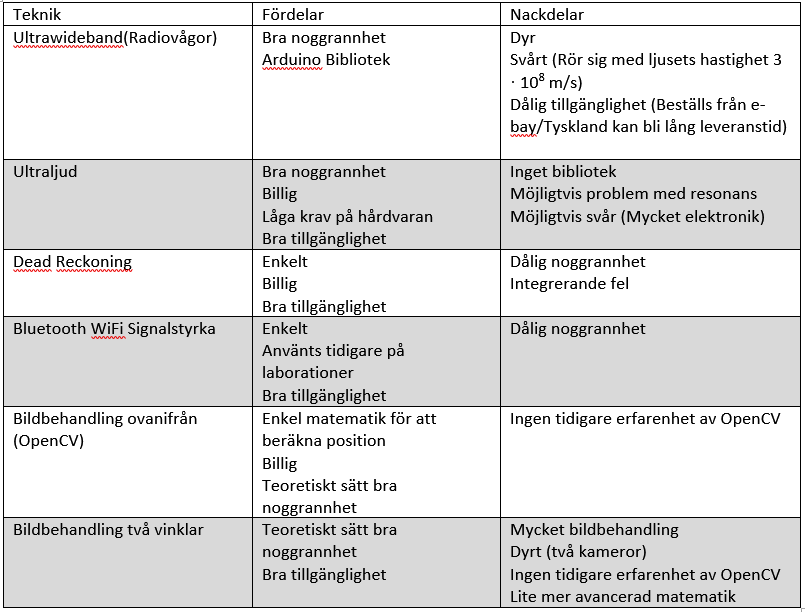
\includegraphics[width=15cm]{genomforbarhetsanalys.PNG}
		\caption{Tabell för genomförbarhetsanalys}
		\label{fig:genomforbarhetsanalys}
	\end{center}
\end{figure}

Resultat

Resultatet av genomförbarhetsanalysen kombinerat med vårt ändamål visar framförallt på att bildbehandlingen och Ultraljuds lösningen är de tekniker som är mest lovande. Eftersom noggrannheten spelar en stor roll, men även tillgängligheten och priset. Till ultraljudslösningen har vi även fått underlag i form av ett exjobb från handledaren. Detta stärker Ultraljudslösningen ytterligare.

\chapter{Metod och utförande}

\section{Problembeskrivning}

\subsection{Behov och egenskaper}

För att bestämma vilken teknologi som kommer att användas till inomhus positionering systemet måste problemet formuleras och krav måste anges. Problemet som skall lösas definieras enligt följande: \\

''Vi vill hitta positionen på ett objekt i ett rum. Positionen skall faställas i ett 2D plan. Eftersom en robot skall kunna hitta till olika objekt  i ett rum behöver den känna till sin position vid given tidpunkt. Objekten kommer att vara mindre hushållsobjekt.'' \\

När problemet är givet kan behov för lösningen definieras. De behov vi identifierat är:

\begin{itemize}
	\item Positionen skall kunna fastställas i realtid.
	\item Noggrannhet skall vara tillräcklig för att en påbyggnad på roboten ska kunna nå objektet.
	\item Systemet skall kunna användas i en offentlig miljö.
	\item Systemet skall fungera i en begränsad plan yta.
	\item Systemet skall fungera oberoende av ljusförhållanden.
	\item Systemet skall ha ett rimligt pris.
	\item Systemet skall kunna kommunicera med roboten.
	\item Systemet för ej vara skadligt.
	\item Systemet får ej vara opålitligt.
\end{itemize}

%% Härnäst skapas en tabell där behoven uttrycks i egenskaper med mätbara enheter.\\
Vi har gjort en tabell där behoven uttrycks i egenskaper med mätbara enheter.\\

\begin{center}
     \begin{tabular}{l | c}
  		Positionen skall fastställas med ett intervall & Hz \\ \hline
        Hög noggrannhet & cm\\ \hline
        Ofarlig & subjektiv\\ \hline
        Möjlig att integrera & subjektiv\\ \hline
        Områden anges med riktlinjer av något slag & subjektiv \\ \hline
        Systemet fungerar i varierande ljusförhållanden & lm \\ \hline
        Inom skolans budget & kr \\ \hline
        Systemet har ett överföringsprotokoll till roboten & subjektiv
  \end{tabular}
\end{center}
\cleardoublepage
För att säkerställa att alla behoven har uppfyllts av egenskaperna skapas en behov-egenskap matris.

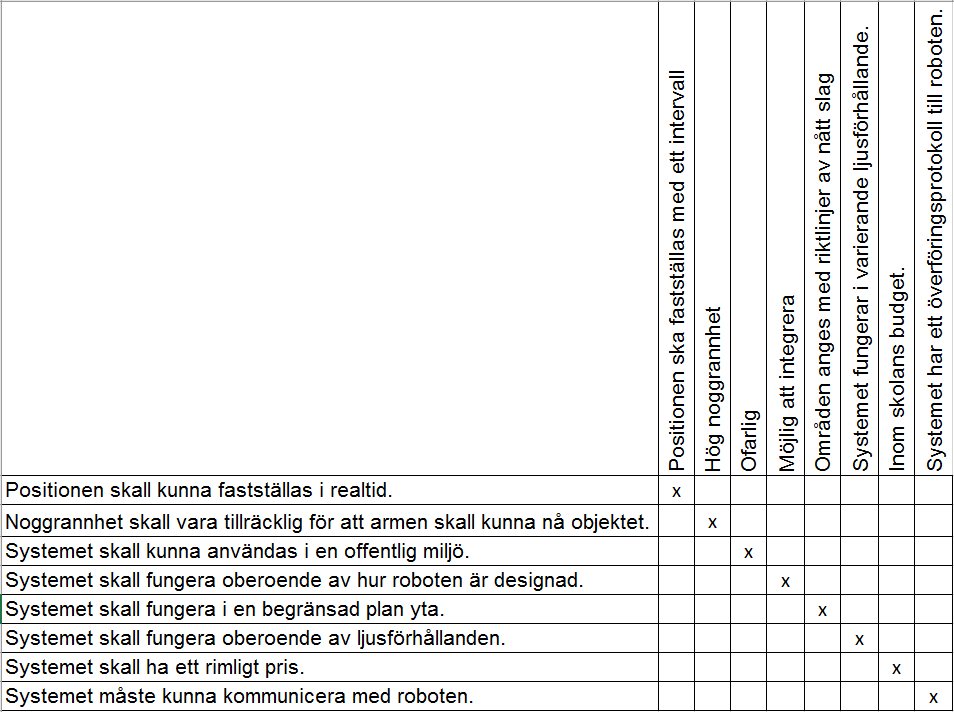
\includegraphics[scale=0.5]{behov-egenskap-matris.PNG}\\
fig \ref{fig:behov-egenskap} \textit{Behov-egenskap matris} %varför är det 9.1???

Som man ser i matrisen uppfylls alla behoven av egenskaperna och därmed är det känt vad en lösning kommer att behöva.

%Systembegrepp bild??


\subsection{Syfte och mål för vår tekniska lösning}
Syftet med den tekniska lösningen är att roboten skall veta var den befinner sig.

Målet med den tekniska lösningen är positionen inte skiljer sig från robotens faktiska position.

% Jag kommenterar ut nästa stycke, tror inte vi ska ha med det...
%% \section{Systemkrav}\label{sec:syskrav}
%% För att utveckla en produkt, i vårt fall ett positioneringssystem, krävs det att innan man börjar sätter upp ett antal krav som man vill att produkten ska uppfylla. Uppgiftsbeskrivningen listar ett fåtal krav och vi har genom diskussion kommit fram till följande kravspecifikation:
%% \begin{itemize}
%% \item Positionen skall kunna fastställas i realtid.
%% \item Noggrannhet skall vara tillräcklig för att armen skall kunna nå objektet.
%% \item Systemet skall kunna användas i en offentlig miljö.
%% \item Systemet skall fungera oberoende av hur roboten är designad.
%% \item Systemet skall fungera i en begränsad plan yta.
%% \item Systemet skall fungera oberoende av ljusförhållanden.
%% \item Systemet skall ha ett rimligt pris.
%% \item Systemet skall kunna kommunicera med roboten.

%% \end{itemize}
%%  Dessa kan sedan översättas till en lista som är är mer lämpad att arbeta utefter:
%%  \begin{center}
%%      \begin{tabular}{ c | c}
%%      	Mätbar Egenskap & Enheter  \\ \hline
%%   		Positionen ska fastställas med ett visst intervall & Hz  \\ \\
%%         Hög noggrannhet & cm\\ \\ 
%%         Ofarlig & subj. \\ \\
%%         Möjlig att integrera & subj.\\ \\
%%         Områden följer förutbestämda riktlinjer & subj\\ \\
%%         Systemet ska fungera i varierade ljusförhållanden & lm\\ \\
%%         Kostnaden ska täckas av skolans budget & kr  \\ \\
%%         Systemet har ett överföringsprotokoll till roboten & subj.\\ 

%%   \end{tabular}
%%   \end{center}

%% Vi kan nu sätta ihop dessa i en s.k. behov-egenskapsmatris som kan ses i bilaga \ref{fig:behov-egenskap}
\subsection{Jämförelse med existerande system}
Vi har i teoriavsnittet tagit upp hur liknande, fast etablerade system, fungerar. Det som skiljer de systemen från vårt är att vårt system har väldigt specifikt användningsområde. Vårt system ska t.ex. inte användas i totalt mörker. Ytan är inte heller dynamisk utan noga uträknad för att kalibrera systemet. Det är alltså inte troligt att vårt system, utan större vidareutvecklingar, hade fungerat i t.ex. ett varuhus. Vi har även endast en användare åt gången vilket förenklar positioneringen något.

\subsection{Systemet och omgivningen}
Vi har identifierat systemets in- och utgångar och visualiserar det i figur \ref{fig:system-omgivning}
\begin{figure}[H]
	\begin{center}
		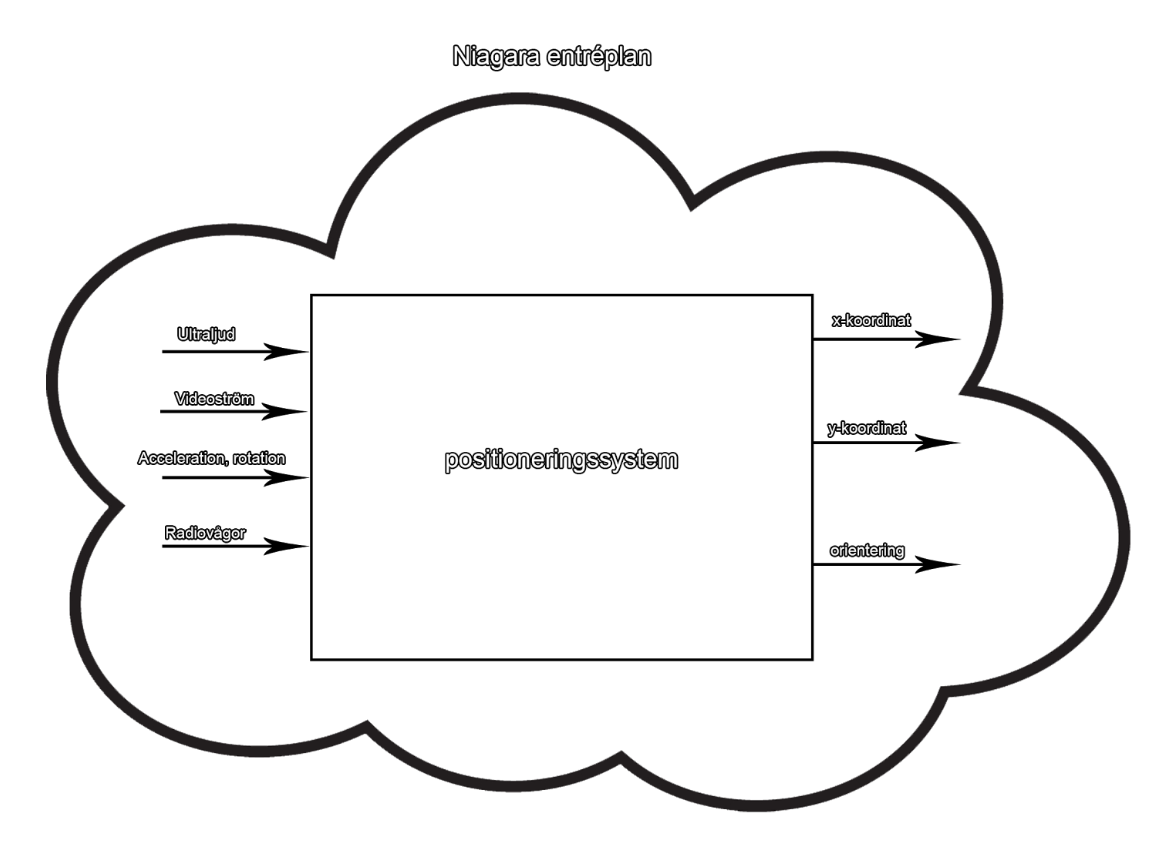
\includegraphics [width=12cm,angle=0]{System-omgivning.PNG}
		\caption{Illutration av systemets in- och utgångar samt dess omgivning}
		\label{fig:system-omgivning}
	\end{center}
\end{figure}

Omgivningen påverkar systemet om det är objekt i vägen då alla ingångar förutom acceleration, rotation påverkas av detta. Systemet påverkas även av störande signaler i omgivningen. Systemets påverkan på omgivningen är i många fall att den skickar ut signaler som stör andra signaler

\clearpage


\section{Hitta och generera lösningskoncept}

\subsection{Huvudproblem och delfunktioner}

Huvudproblemet i vårt fall, att kunna fastställa positionen på ett objekt i ett rum, har vi formulerat om lite mer abstrakt och översiktligt till inomhusposition eftersom det är exakt detta systemet skall uppnå. Huvudproblemet bröt vi sedan ned i tre olika delfunktioner som även de var abstrakta och översiktliga.

\begin{figure}[H]
	\begin{center}
		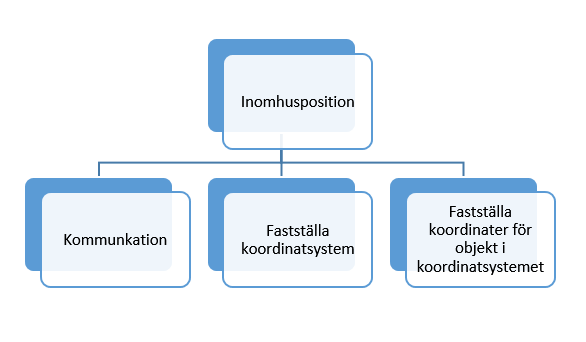
\includegraphics [width=12cm,angle=0]{delfunktioner.PNG}
		\caption{Huvudproblemet och dess delfunktioner}
		\label{fig:huvudproblem}
	\end{center}
\end{figure}


\subsection{Delfunktioner och lösningsprinciper}

Delfunktionerna visas ovan och till dessa har vi sedan försökt hitta olika lösningsprinciper genom olika metoder så som '365'-metoden och 'sex tänkande hattar'. Eftersom vårt problem är relativt avancerat så har vi kapat bort lite lösnings principer som är för avancerade och tokiga då det måste finnas en rimlighetsfaktor. De olika delfunktionerna och de olika lösningprinciperna illusteras i bilaga \ref{fig:koordinatsystem} - \ref{fig:kommunikation}.

\subsection{Funktion- och medelträd}

Detta trädet illustrera huvudproblemet och underfunktionerna där underfunktionerna har kombinerats ihop med dess olika lösningsprinciper. Bilaga \ref{fig:funktionmedel} visar funktion/medel-trädet.


\subsection{Ordningsprincip}

Nedan är en skiss på hur huvudfunktionen ser ut när vi valt ut dem lösningsprinciper som vi anser vara 'bäst'. \\


\begin{figure}[H]
	\begin{center}
		\includegraphics [width=12cm,angle=0]{Blockdiagram.png}
		\caption{Skiss av konceptet med hjälp av olika lösningsprinciper}
		\label{fig:blockdiagram}
	\end{center}
\end{figure}

Bildbehandlingen är starkt beroende av att vi faktiskt mätt upp och bestämt ett koordinatsystem i rummet, annars går det ej att bestämma positionen med hjälp bildbehandlingen. Däremot är SPI-kommunikationen inte tekniskt beroende av bildbehandlingen och koordinatsystemet. Men utan deras bidrag har kommunikationsdelen ingen data att skicka, och därför ser vi den som beroende av de andra blocken.

Ordningen är kritiskt vilket framgår av blockschemat, skulle det göras i en annan ordning skulle det ej fungera. 


\subsection{Förflyttning och provokation metoden}

Tanken med förflyttning och provokation är att skapa ännu fler möjliga lösingsprinciper genom att modifiera, invertera och skapa störningar och extremfall utifrån blockdiagrammet som gjordes i föregående steg. 

Negation:
Vi väljer att ta bort delen “bildbehandling” och ersätter den med ett antal nya idéer:

Snöre:
Man skulle kunna ha ett snöre på en rulle som sitter på en ledad arm. Beroende på hur mycket snöre som har rullat ut och i vilken riktning det hade rullats ut så skulle man kunna beräkna positionen med hjälp av de parametrarna.
Konceptuellt en enkel idé men kan vara svår att bygga så att den blir tillräckligt känslig.

WiFi/Bluetooth: 
Man har t.ex. tre sändare utplacerade på golvet och en mottagare placerad på roboten och avgör sedan positionen genom att mäta signalstyrkan till de olika sändarna. 
Hade kunnat fungera någotsånär, men vi har märkt på laborationer i tidigare kurser att bluetooth signalstyrkan är väldigt känslig för störningar och ger inte så exakta värden. Det samma gäller för wifi. Med tanke på hur mycket wifi-signaler som finns i Niagara så kan det bli svårt att få en bra positionering med detta system.

Bildbehandling två vinkar:
Originaltanken med bildbehandlingen var att ha en kamera som filmar banan ovanifrån och beräknar positionen med hjälp av detta. Ett alternativ till detta är att man istället använder två kameror från olika vinklar istället fastställer koordinaterna med hjälp av triangulering.

Radiovågor och Ultraljud:
Principen för dessa tekniker är ungefär samma, att objektet har en mikrofon (ultraljud) / mottagare (radiovågor) för att sedan bestämma tiden det tar för ultraljudet alternativt radiovågorna att nå objektet. Då kan man bestämma sträckan och med hjälp av trilaterering även positionen.


Inversion:

Tanken vi hade med inversion var att man inverterar kommunikationen, d v s roboten kommunicerar med vårt inomhuspositionering system istället för att vi informerar roboten om var den befinner sig. Då skulle roboten behöva kommunicera hur mycket den har rört sig, vilken riktning m.m för att vårt system ska kunna räkna ut var roboten befinner sig. Detta skulle faktiskt vara ett realistiskt scenario, problemet som kan uppstå är att noggrannheten blir väldigt dålig. Ett integrerande fel om ingen kalibrering utförs.

Man skulle även kunna invertera bildbehandlingen till ljud, så man har någon form av ljud som säger till roboten var den befinner sig och roboten lyssnar på dessa ljuden och på så sätt vet roboten var den befinner sig. 

Extremfall:

I vårt fall är det svårt att avgöra vad ett extremfall skulle vara. Ett extremfall kan ju t ex vara att positionen ska kunna fastställas i ett väldigt stort rum istället för på en liten yta, då skulle många lösningsprinciper för att fastställa positionen på objekt falla bort. Exempelvis skulle lösningar med kamera inte fungera då det blir väldigt problematiskt att filma hela rummet. Lösningar med elektromagnetiska vågor, radio eller ljus t ex, blir då lämpligare, då de lätt rör sig över stora ytor.

Man kan även vända på pannkakan och säga att man ska bestämma positionen på en extremt liten yta, d v s molekyl/atomnivå. Det svårt att komma på lösningsprinciper för denna typen av problem, men eventuellt hade man kanske kunnat kolla på strukturen av atomerna och molekylerna för på så sätt kunna bestämma positionen. Beroende på materialet så har ju atomerna en viss struktur/mönster vilket kanske kan omformuleras till en position på något kreativt sätt.


Störning:

Störning i detta sammanhang innebär att man genom att ändra ordning på blocken i diagrammet ovan utvärdera om den ordning man satt upp verkligen är nödvändig, samt se om nya ideer uppstår. Den störning vi diskuterat är att ändra ordning på bildbehandlingen och uppmätning av koordinatsystemet. Då kan man tänka sig ett system där vi filmar en yta med en kamera, och för varje punkt vi är intresserade av kontrollerar vilken pixelkoordinat den har i bilden vi filmat. Detta system hade kunnat fungera, och ha den fördelen mot vår existerande ide att den inte förlitar sig på någon geometrisk omräkning, vilken kan introducera fel. Nackdelen är att vi måste hårdkoda samtliga koordinater vi är intresserade av, vilket leder till mycket jobb, ett visst mått av trial and error samt en lägre upplösning av punkter.

Byter vi plats på kommunikation och de övriga delarna så händer inte så mycket och det inspirerar inte så mycket nya lösningar eftersom den enda konsekvensen blir att systemet blir icke fungerande. Då kommunikationen måste ske sist, annars har vi ingen att kommunicera, d v s saker utförs inte “rätt” ordning.


\subsection{Uppdaterat funktions/medel-träd}

Förflyttning och provokation genererade många nya möjliga idéer och lösningsprinciper utifrån blockschemadiagrammet. Därför strukturerade vi om vårt funktion- och medelträd där vi skapat underfunktioner till delfunktionerna för att kategorisera de olika lösningsprinciperna. Bilaga \ref{fig:funktionmedel2} visar det uppdaterade funktions/medel-trädet.

Det nya funktions/medel-trädet visas även med hjälp av en konceptkombinationstabell där varje underfunktion kombineras med lösningsprinciperna som associeras till underfunktionen. Tabellen finns i bilaga \ref{fig:koncepttabell1}.


\subsection{Morfologiska matriser}

När vi tog fram de morfologiska matriserna utgick vi från konceptkombinationstabellen som vi skapade i föregående avsnitt. Det vi gjorde var att ta bort lösningar som inte var aktuella av olika anledninger, t ex att de är svåra att genomföra, ger dåligt resultat, är dyra, etc. Detta gav oss en ny matris som går att se i bilaga \ref{fig:koncepttabell2}. Den nya matrisen genererade 60 olika möjliga lösningskombinationer att välja på. De olika lösningskombinationerna bedöms om de uppfyller huvudproblem, men även kraven på systemet. En något för kortad matris med bedömningen går att se i bilaga \ref{fig:hpk}.

\section{Utvärdering av lösningsvarianter}

\subsection{5 mest lovande lösningsvarianter}

Utifrån den morfologiska matrisen med bedömning om vilka lösningsvarianter som uppfyller huvudproblemet samt kraven så valde vi ut de 5 mest lovande lösningsvarianterna. Vilka lösningsvarianter detta är och beskrivning av dem visas i bilaga \ref{fig:5koncept}.


\subsection{Kriterier och viktning}

Kriterierna är valda dels efter våra egna uppsatta krav, dels med kraven från uppgiftsbeskrivningen. 
\begin{itemize}
\item \textbf{Noggrannhet:}
För att klara uppgiften i projektet är det kritiskt att robotarna vet var de befinner sig, samt var vissa objekt befinner sig, inom en viss felmarginal, som gärna ska vara liten. Därför är noggrannhet ett viktigt kriterium för vår lösning. Vi har delat upp kriteriet i två delar, precision och uppdateringsfrekvens, och fördelat vikten för noggrannhet jämnt över dessa två delkriterier.

\item \textbf{Offentlig miljö:}
Detta kriterium är uppdelat i två delkriterier - att systemet ska vara ofarligt för allmänheten och att systemet ska fungera med publik på plats. Vi har givit det relativt låg vikt då vi i någon mån kommer kunna kontrollera platsen för demonstrationen, samt att förutom begränsningen att vi inte ska använda laser så har vi inte haft några hälsovådliga tekniker på förslag.

\item \textbf{Pris:}
Pris valde vi som ett kriterium eftersom det är väldigt relevant att lösningsvarianter inte får kosta för mycket, viss utrustning vi har kollat på är väldigt dyr och detta måste då vara med och viktas in i bedömningen om vilket teknik som är mest lämplig. Viktningen av detta kriteriet baseras på den information om kostnader vi har hittat när vi titta på de olika teknikerna. Det är endast ett fåtal tekniker som är för dyra att implementera, därför är viktningen relativt låg.

\item \textbf{Implementering:}
Detta kriterium avspeglar hur komplicerat det är att genomföra (implementera) olika lösningar, vilket är av vikt då tiden för projektet är begränsat.
Genom att ändra på vikten på detta kriterium så får man en bra känsla vad som är lämpligt som ett enklare respektive avancerat system. Detta kriteriet fick en ganska stor viktning eftersom det är väldigt begränsat med tid och därav är väldigt viktigt att vi inte ger oss på något som är för svårt.

En tabell med kriterier och viktning finns i bilaga \ref{fig:kriteriumvikt}

\end{itemize}

\subsection{Bedömning av kriterier}

Kriterierna har vi sedan gett en bedömningsskala som är samma för alla kriterium. Om viktningen ska ha någon inverkan är det viktigt att samtliga kriterier bedöms med samma skala, annars är det meningslöst med viktningen.

Bedömingsskalan och kriterier finns i bilaga \ref{fig:bedomningskala}

\subsection{Bedömning av lösningsvarianterna för varje kriterium}

I tabellen i bilaga \ref{fig:medbedomning} är lösningsvarianterna betygsatta enligt en rad olika kriterier på en skala 1-10, summan av betygen för varje lösningsvariant framgår på sista raden. Detta gör vi som ett steg i arbetet att systematiskt utvärdera olika lösningar.

\subsection{Poängsättningsmatris}

Utifrån tabellen med bedömningen av de olika lösningvarianterna har vi sedan multiplcerat bedömningen med viktningen av de olika kriterierna. Detta gör vi för att kriterierna skall bedömas med den vikt vi anser att kriterierna har. Poängsättningsmatrisen går att se i bilaga \ref{fig:bedomningvikt}

\subsection{Känslighetsanalys}

I detta steg ändrar vi viktningen av de olika kriterierna. Det vi vill se är om samma lösningsvariant ändå ger bäst resultat, eller om en annan visar sig bäst. Vi kan på så sätt få insikt i hur robusta de olika varianterna är, och vi kan ju inte vara säkra på att bedömningen och viktningen vi gjort är korrekt. Detta ger oss mer kontext för att komma fram till bästa lösningsvarianten. I bilaga \ref{fig:rangordning} går det att se resultatet från känslighetsanalysen, där vi har gjort 3 olika varianter av viktningen och bedömning.

\subsection{Vinnande koncept}

Vi kommer att skapa två system, ett enklare och ett avancerat system. Därför korar vi två vinnare, LV3 och LV1. Då implementationen är viktat högt i variant A så vinner LV1, d v s detta system anser vi vara ett rimligt enklare system. Vid en senare tidpunkt när vi har ett enklare fungerande system försöker vi göra ett lite mer avancerat vilket då blir LV3.


LV1 -

Kameralösningen är en väldigt smidig lösning då den är relativt enkel att skapa och den ger en noggrannhet som är tillräckligt bra. Lösningen använder bara en sensor vilket då är kameran.
Kameran kommer att skicka video till en dator som sedan behandlar bilden och tar ut positionen. Positionen skickas sedan trådlöst till en mottagare på roboten som meddelar via SPI till robotens styrsystem var den befinner sig. Systemet är väldigt energisnålt när det gäller det som går på batteri, allt som behöver drivas är en ESP8266 samt några lysdioder. Det kommer att vara publik runt om banan som kanske inte vill hamna på video, vilket kan innebär ett integritetsproblem.


LV3 -

Lösningsvarianten med ultraljud fungerar genom att vi sätter upp två till tre ultraljudshögtalare inom ett bestämt område. Vi monterar sedan en eller flera mikrofoner på roboten och mäter sedan hur långt ifrån roboten är från vardera högtalare genom att mäta hur lång tid det tar innan ljudet från högtalarna når roboten.

Lösningen kräver som sagt två till tre ultraljudshögtalare med något stativ. Två till tre mikrofoner som ska monteras på roboten, samt två Arduino Due, en som samplar ljud monterad på roboten och en Due som skapar signalen som skickas ut genom högtalarna.
Det som är kritiskt är att mikrofonerna måste monteras på en plats på roboten som inte skyms av armar och andra hinder på roboten.
Det enda som behöver ström från roboten är alltså ett Arduino Due utvecklingskort.


I de båda lösningarna så är det endast SPI kommunikation som är utgången från vårt navigeringssystem. Det är alltså endast detta som resterande grupper behöver ta hänsyn till för att lösa överföringen av koordinater till deras styrsystem.

\section{Diskussion och resultat}

LV1 -

LV1 vann på grund av att det är lättare att implementera än en ultraljuds lösning, detta syntes tydligt när viktningen på implementering ändrades. Detta är en prioritet för inför M2 att implementationen inte är för svår. Detta är den mest utmärkande egenskapen med denna lösningen och bidrog mest till att den vann. 

LV3 -

LV3 vann på grund av att det är noggrannare än en kamera lösning, teoretiskt sätt kommer ultraljuds lösningen att ha en centimeter noggrannhet. Detta systemet kommer vi att skapa som det avancerade systemet och skall vara klart mot slutet av projektet.



Vad var svårt, nytt och ovant?

Det svåraste med den tredje delen av den tekniska problemlösningen var nog valet av bra kriterier samt viktningen av dessa. Det är ju viktigt att här välja ut bra och relevanta krav som vi tycker att systemet ska uppfylla, för att i slutändan få det bästa alternativet av de många koncept vi tidigare har genererat.


Hur lika eller olika var bedömningen mellan gruppmedlemmarna?

Som grupp var vi på samma nivå med bedömningen, vi har tittat lite på de olika teknikerna som lösningsförslagen involverar sedan tidigare och har erfarenhet av några. Bedömningen har alltså gjorts utifrån detta, på lösningsförslagen som är osäkra har vi försökt göra en rimlig bedömning tillsammans som grupp för att alla skall vara överens.

Blev ni förvånade av att rangordningen blev som den blev?

När vi väl hade den slutgiltliga listan på 5 utvalda koncept, så kunde man relativt lätt tänka sig ungefär vilka placeringar som var och ett av dem skulle få. Detta eftersom att vi visste att SPI skulle vara mycket lättare att implementera än I2C och att radiovågor lösningen skulle bli väldigt dyr.

Hade ni några favorit lösningar och landade någon av dem på första plats?

Våra favorit lösningar var kameralösning, ultraljuds lösning samt en pratande robot. Kamera lösningen och ultraljuds lösningen hamnade på första plats och de är de vi kommer att använda. De var våra favoriter eftersom båda känns rimliga att göra, kamera lösningen bör vara ganska enkel samt att ultraljuds lösningen får väldigt bra noggrannhet.

Ändrade sig rangordningen under känslighetsanalysen?

Som tidigare nämnts så var det bildanalyslösningen och ultraljudslösningen som skiftade plats då vi ändrade på viktningen av våra kriterier. Detta passade oss dock endast bra eftersom vi var ute efter ett lite lättare system och ett som var mer avancerat, vilket representeras bra av de båda koncepten. 


\section{Testning}
För att se till att systemet som har utvecklats verkligen fungerar måste det testas. Sättet att gå till väga för att testa systemet är att fastställa vilka krav som ställs på systemet för att sedan se till att dessa krav uppfylls. Kraven som detta positioneringssystem har beskrivs enligt:

\begin{center}
	\begin{tabular}{c | p{13.5cm}}
	ID & Systemkrav på högsta nivå \\ \hline
	K1 & Systemet skall kunna fastställa position för objekt i koordinatsystem. \\
	K2 & Fastställa ett koordinatsystem på bottenvåningen i Niagara där robotarna utför sin uppgift, som är minsta 5 x 4 m stort. \\
	K3 & Systemet skall kommunicera den uppmätta positionen via ett givet väldefinierat elektroniskt kommunikationsprotokoll \\
	\end{tabular}
	\\ [0.5cm]
\end{center}

	Systemkrav på högsta nivån är krav som säger vad systemet skall kunna göra. För detta positioneringssystem är många aspekter givna i förväg såsom var det skall användas och under vilka förhållanden och utifrån det har vi tagit fram specifika krav.
	
\begin{center}
	\begin{tabular}{c | p{13.5cm}}
	ID & Icke funktionella krav \\ \hline
	K4 & Systemet skall vara ofarligt \\
	K5 & Ultraljudssystemet får inte använda frekvenser som kan störa eller störas av kringliggande utrustning såsom avståndsmätare eller PWM-signal. \\
	K6 & Positionsdata presenteras enligt ett fördefinierat format. \\
	\end{tabular}
	\\ [0.5cm]
\end{center}

Icke funktionella krav är krav som inte uppfyller någon funktion, alltså inte lägger till någon ny funktion. Dessa krav är mer prestanda krav som säger hur bra systemet skall klara andra krav.

\begin{center}
	\begin{tabular}{c | p{13.5cm}}
	ID & Funktionella systemkrav på de komponenter som ingår \\ \hline
	K7 & Modul och python program kan kommunicera med server \\
	K8 & Noggrannheten är högre än 30 cm / 10 cm, där noggrannheten innebär avståndet mellan faktiskt läge och det läge systemet anger. \\
	K9 & Uppdateringsfrekvensen är minst 1 Hz. \\
	K10 & Pixlars position kan mappas mot en fysisk position. \\
	K11 & Kommunikation mellan Due och ESP fungerar \\	
	\end{tabular}
	\\ [0.5cm]
\end{center}

Funktionella systemkrav på de komponenter som ingår är krav som ställs på enskilda delar av systemet.

\begin{center}
	\begin{tabular}{c | p{13.5cm}}
	ID & Andra krav på komponenter \\ \hline
	K12 & Utvecklingskortet på roboten har stöd för det valda kommunikationsprotokollet. \\
	K13 & OpenCV programmet kan hitta koordinaterna för en lysdiod i en bild \\	
	\end{tabular}
	\\ [0.5cm]
\end{center}

Andra krav på komponenter är icke funktionella krav som ställs på komponenter i systemet och inte systemet i helhet. Dessa kan tex vara krav på hårdvarukomponenter.

\begin{center}
	\begin{tabular}{c | p{13.5cm}}
	ID & Krav på gränssnitt \\ \hline
	K14 & Kommunikationsprotokollet skall kunna överföra ett meddelande på 8 byte. \\
	K15 & Montering skall finnas för lysdioder samt mikrofoner på roboten med Line of Sight \\	
	\end{tabular}
\end{center}

Krav på gränssnitt innebär krav på hur vårt system interagerar med andra system. I vårt fall kommer det att vara mot självaste roboten.

Med alla dessa krav kan som sagt systemet testas och det görs genom olika testfall. Varje testfall skall då testa en eller mer del i systemet genom tydliga instruktioner. Det är viktigt att testfallen är skrivna på ett sätt så att resultatet inte är subjektivt. Oavsett vilken person som testar systemet så skall resultatet på testet bli samma. De testfall som har definierats för detta system kan ses i bilaga \ref{fig:testfall}.


\chapter{Resultat}
Vi kommer att klargöra vilka teknologi/er vi har valt för vår lösning och varför som resultat av vår konceptstudie.

Beskrivning av hur, vårt nu fungerande positioneringssystem, fungerar. 

\chapter{Diskussion}
\begin{itemize}
\item Vad gick bra, vad gick som vi hade tänkt oss?
\item Hur fungerar vårt system jämfört med andra som finns och varför?
\item Hade det gått att använda vårt system i större skala?
\end{itemize} 




\chapter{Slutsats}
Vi gör här en kort summering av arbetet.
Samt:
Vilka slutsatser kan vi dra från resultatet och projektet i stort?
Vad har vi lärt oss?






\newpage
\begin{thebibliography}{99}

\bibitem{Tom} Tom

\end{thebibliography}

\chapter{Bilagor}
Vi kommer här att lägga bilder och ekvationer samt eventuella länkar som hindrar läsbarheten och bara tar plats i texten.

\begin{figure}[H]
	\begin{center}
		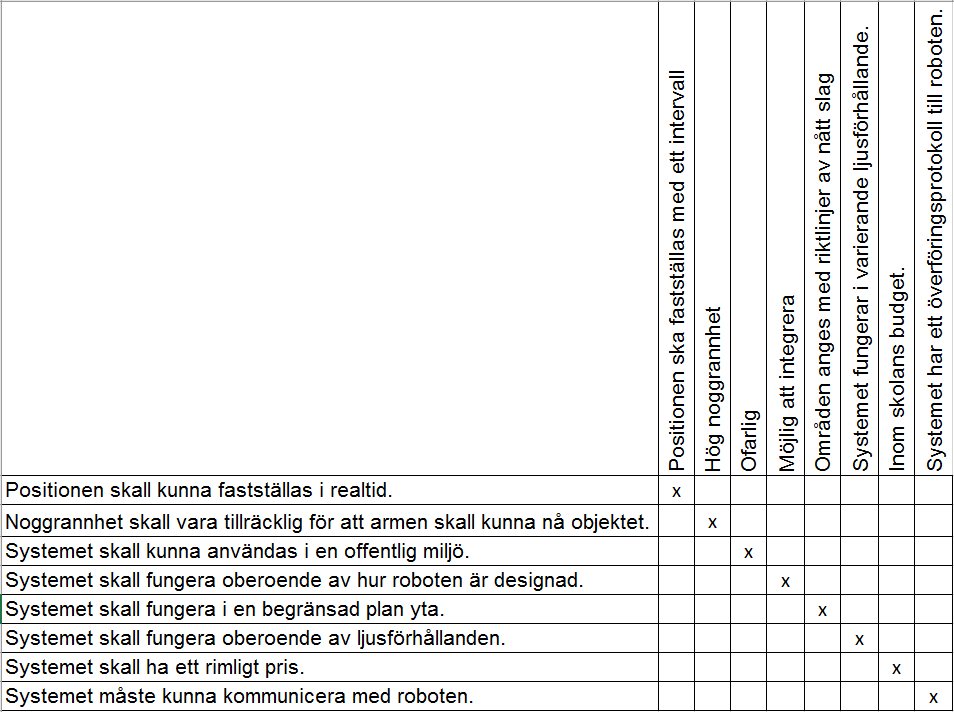
\includegraphics [width=12cm,angle=0]{behov-egenskap-matris.PNG}
		\caption{Behov-egenskapsmatris}
		\label{fig:behov-egenskap}
	\end{center}
\end{figure}


\begin{figure}[H]
	\begin{center}
		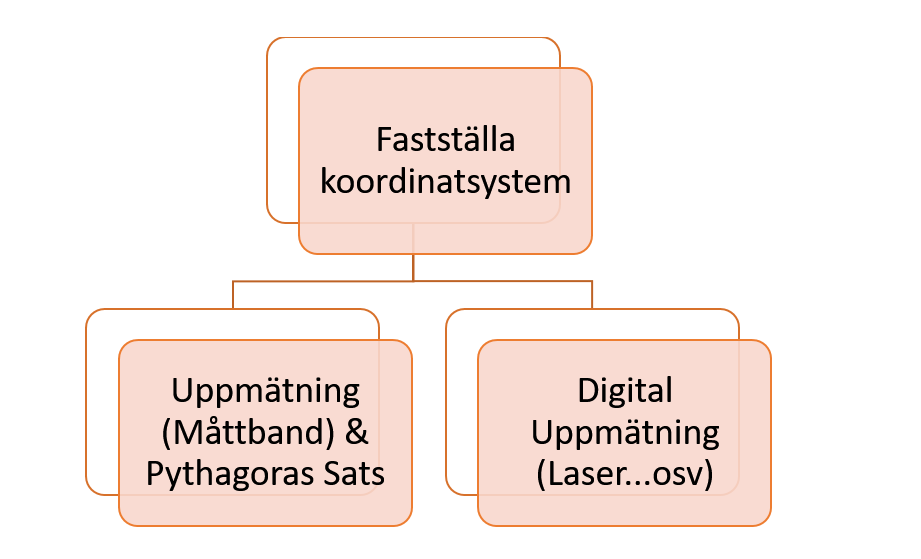
\includegraphics [width=12cm, height=7cm, angle=0]{faststallakoordinatsystem.PNG}
		\caption{Delfunktion fastställa koordinatsystem med lösningsprinciper}
		\label{fig:koordinatsystem}
	\end{center}
\end{figure}

\begin{figure}[H]
	\begin{center}
		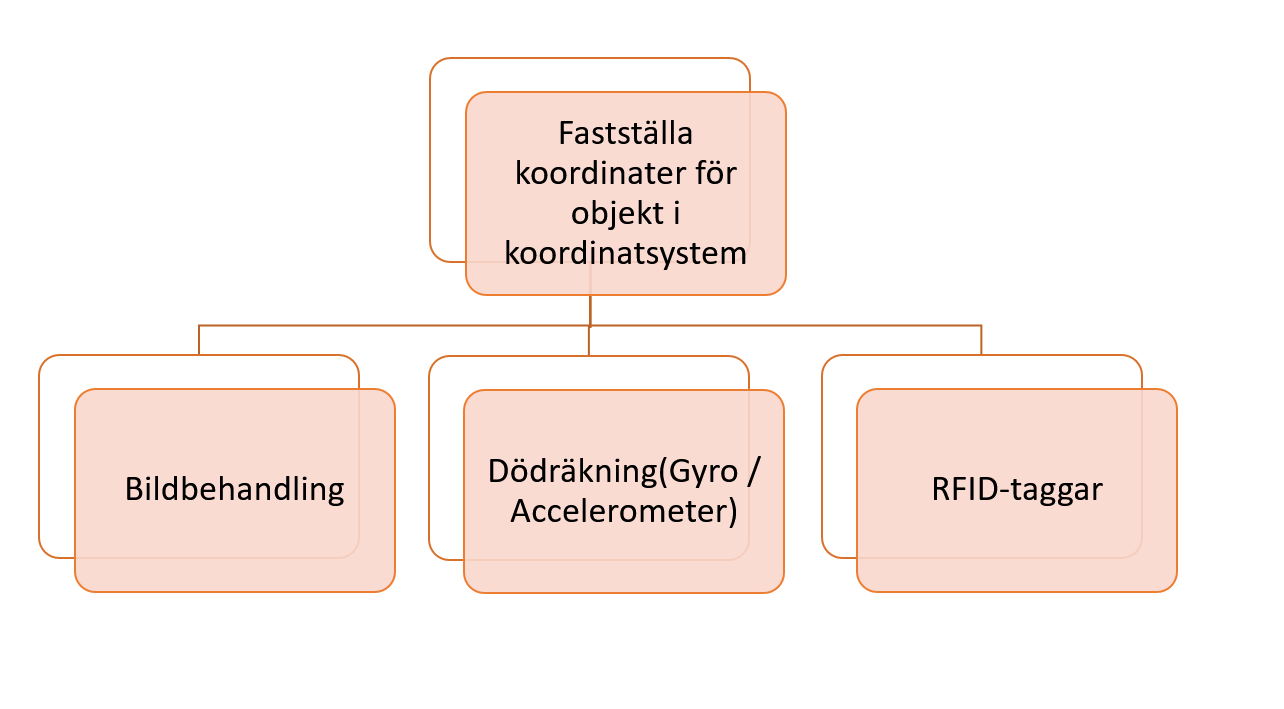
\includegraphics [width=12cm, height=7cm, angle=0]{objekt.PNG}
		\caption{Delfunktion fastställa koordinater med lösningsprinciper}
		\label{fig:objekt}
	\end{center}
\end{figure}


\begin{figure}[H]
	\begin{center}
		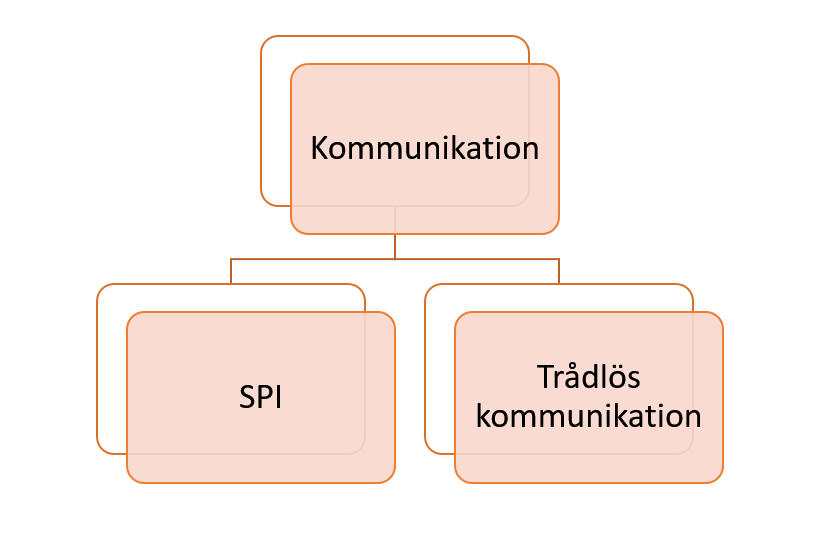
\includegraphics [width=12cm,height=7cm,angle=0]{kommunikation.PNG}
		\caption{Delfunktion kommunikation med lösningsprinciper}
		\label{fig:kommunikation}
	\end{center}
\end{figure}


\begin{figure}[H]
	\begin{center}
		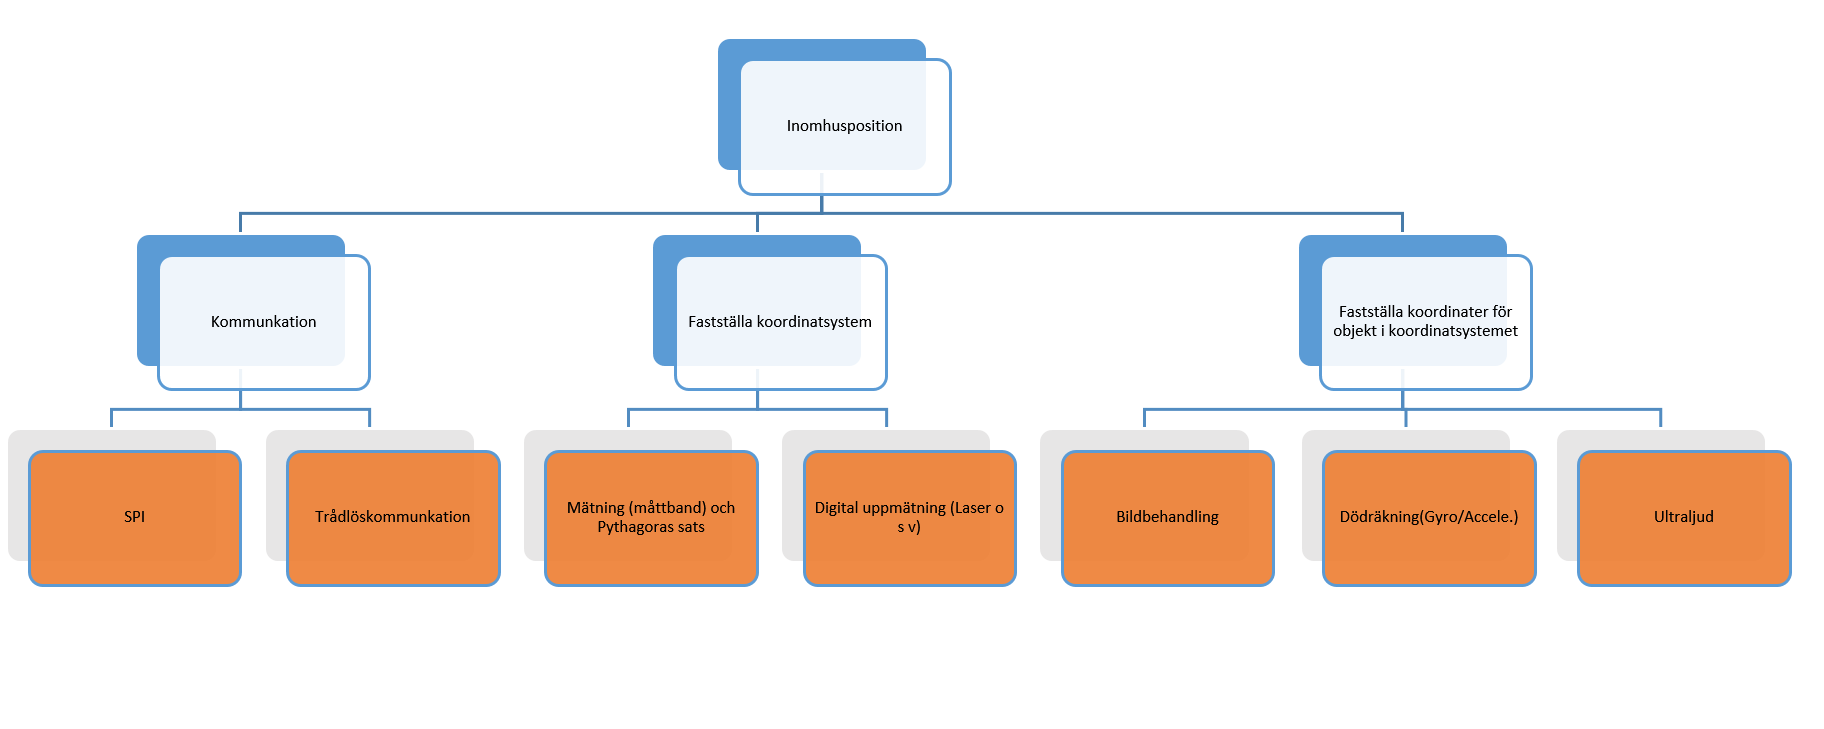
\includegraphics [width=12cm,angle=0]{funktionmedel.PNG}
		\caption{Delfunktion kommunikation med lösningsprinciper}
		\label{fig:funktionmedel}
	\end{center}
\end{figure}

\begin{figure}[H]
	\begin{center}
		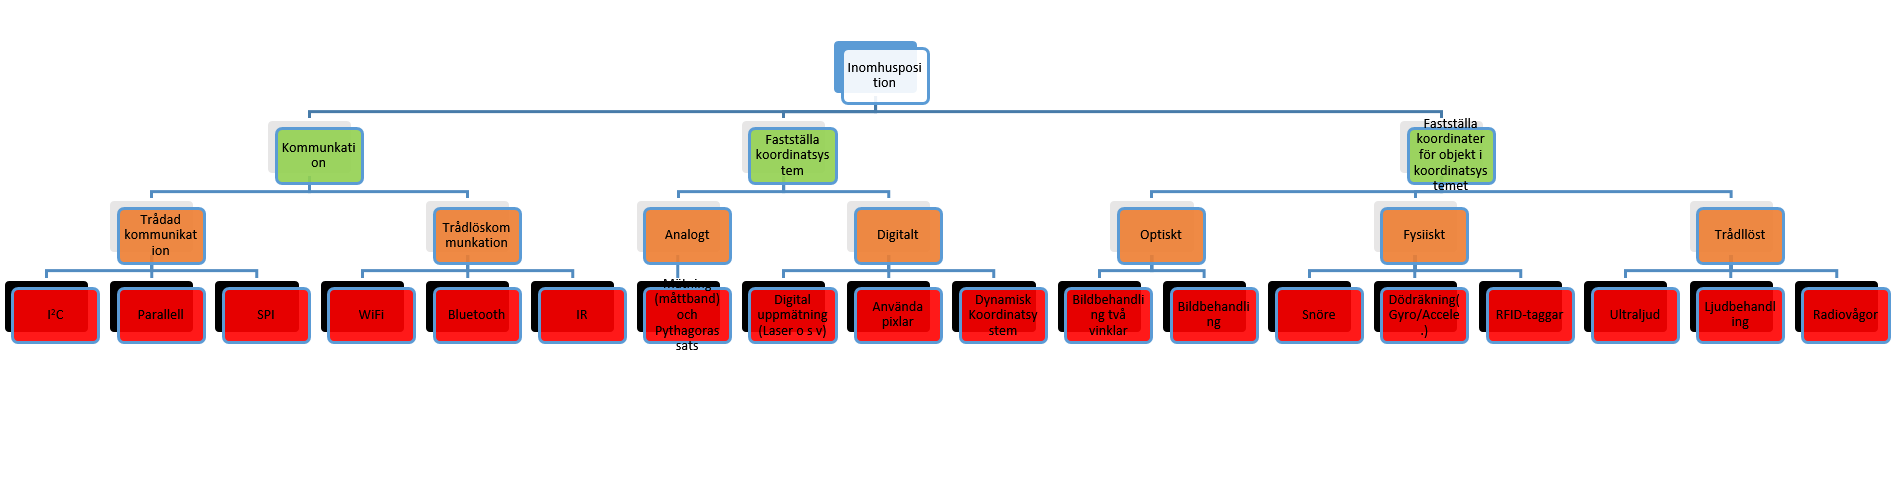
\includegraphics [width=12cm,angle=0]{funktionmedel2.PNG}
		\caption{Nytt funktion/medel-träd}
		\label{fig:funktionmedel2}
	\end{center}
\end{figure}

\begin{figure}[H]
	\begin{center}
		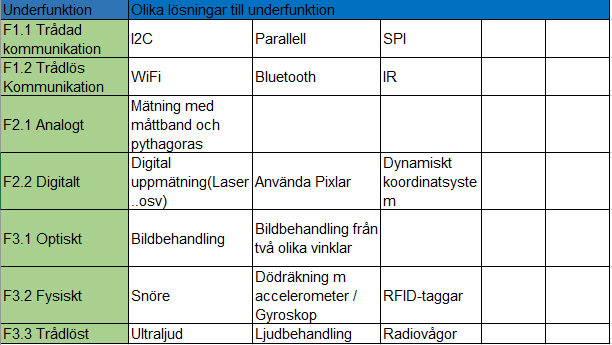
\includegraphics [width=12cm,angle=0]{konceptkombtabell.PNG}
		\caption{Konceptkombinationstabell}
		\label{fig:koncepttabell1}
	\end{center}
\end{figure}


\begin{figure}[H]
	\begin{center}
		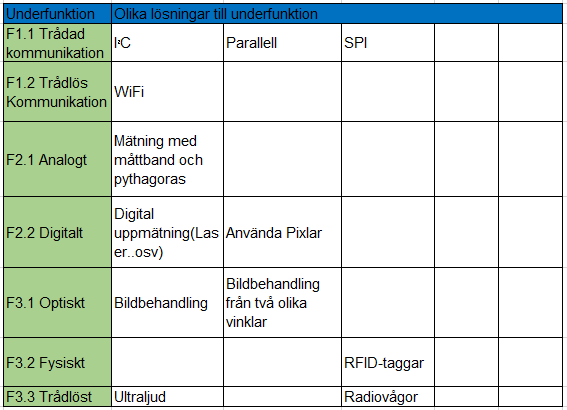
\includegraphics [width=12cm,angle=0]{trimmadtabell.PNG}
		\caption{Trimmad konceptkobinationstabell }
		\label{fig:koncepttabell2}
	\end{center}
\end{figure}

\begin{figure}[H]
	\begin{center}
		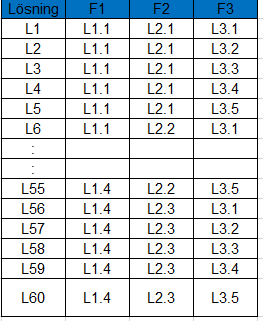
\includegraphics [angle=0]{Losningsforslag.PNG}
		\caption{Möjlig lösningskombinationer }
		\label{fig:mojligalosningar}
	\end{center}
\end{figure}


\begin{figure}[H]
	\begin{center}
		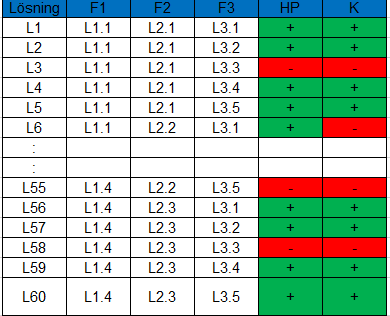
\includegraphics [width=12cm,angle=0]{HPK.PNG}
		\caption{Möjliga lösningskombinationer som uppfyller krav och huvudproblem }
		\label{fig:hpk}
	\end{center}
\end{figure}

\begin{figure}[H]
	\begin{center}
		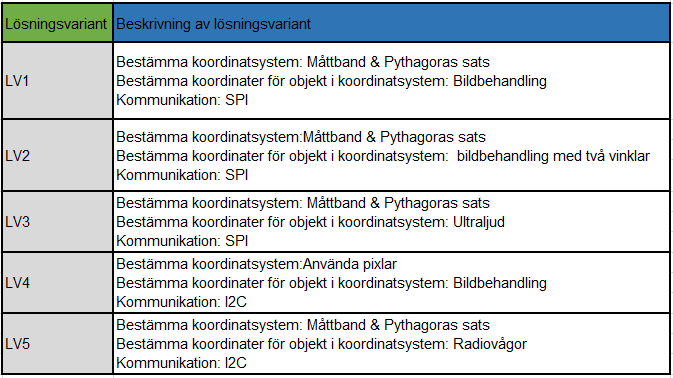
\includegraphics [width=12cm,angle=0]{5koncept.PNG}
		\caption{De 5 mest lovande lösningsvarianterna }
		\label{fig:5koncept}
	\end{center}
\end{figure}


\begin{figure}[H]
	\begin{center}
		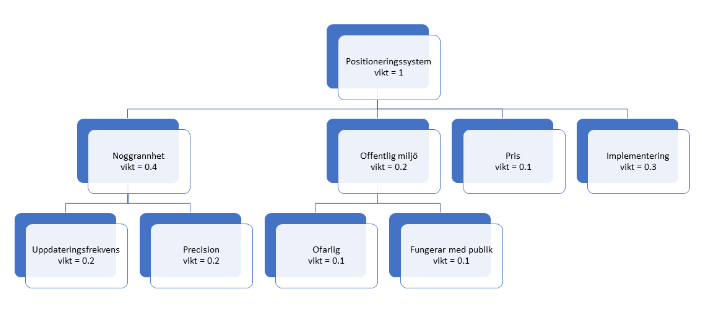
\includegraphics [width=12cm,angle=0]{kriteriumvikt.PNG}
		\caption{Kriterium med viktning }
		\label{fig:kriteriumvikt}
	\end{center}
\end{figure}

\begin{figure}[H]
	\begin{center}
		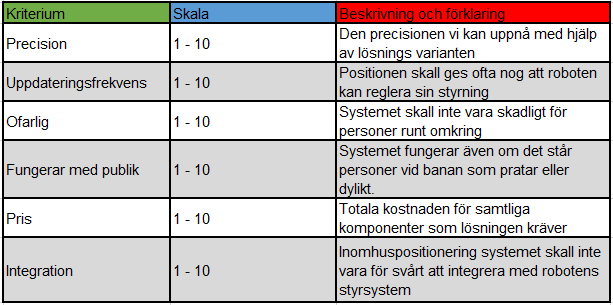
\includegraphics [width=12cm,angle=0]{bedomningskala.PNG}
		\caption{Kriterium med bedömningsskala }
		\label{fig:bedomningskala}
	\end{center}
\end{figure}

\begin{figure}[H]
	\begin{center}
		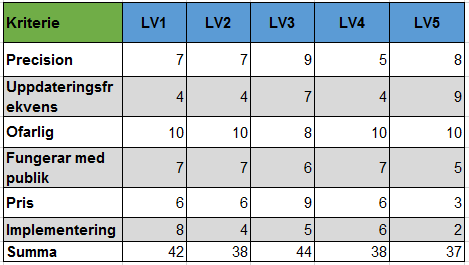
\includegraphics [width=12cm,angle=0]{bedomningavkrit.PNG}
		\caption{Lösningsvarianter med bedömning}
		\label{fig:medbedomning}
	\end{center}
\end{figure}

\begin{figure}[H]
	\begin{center}
		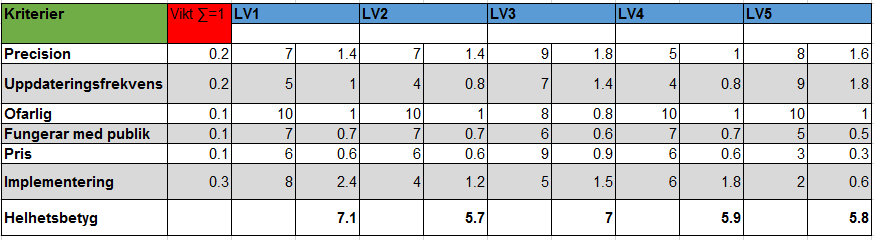
\includegraphics [width=12cm,angle=0]{bedomningvikt.PNG}
		\caption{Lösningsvarianter med bedömning samt viktning av de olika kriterierna}
		\label{fig:bedomningvikt}
	\end{center}
\end{figure}

\begin{figure}[H]
	\begin{center}
		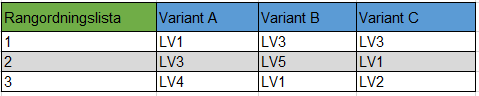
\includegraphics [width=12cm,angle=0]{rangordning.PNG}
		\caption{Känslighetsanalys varation av viktningen}
		\label{fig:rangordning}
	\end{center}
\end{figure}

\begin{figure}[H]
	\begin{center}
		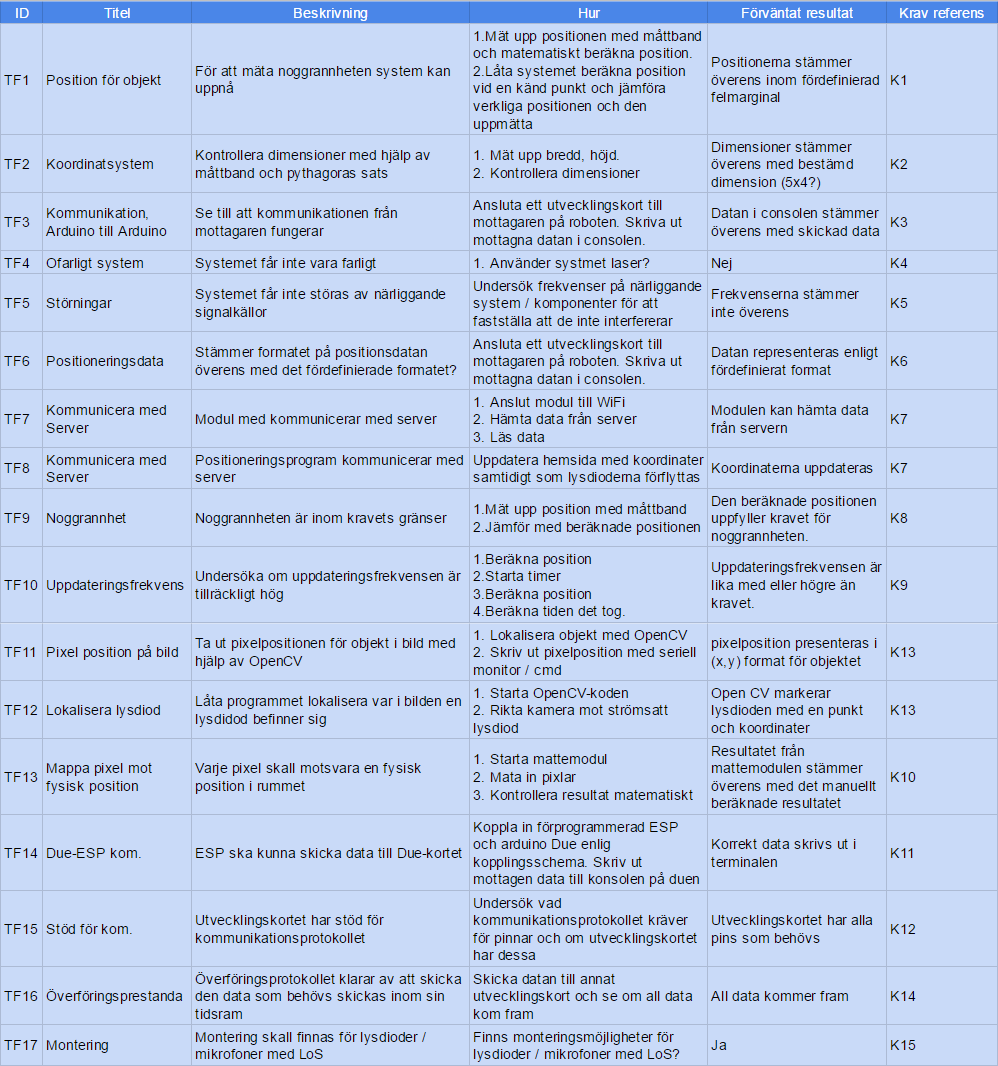
\includegraphics[width=15cm]{systemkrav.PNG}
		\caption{Testfall}
		\label{fig:testfall}
	\end{center}
\end{figure}
\end{document}
